\section{Dise�o de estructura de sistema}

En la Figura~\ref{fig:diagrama_general} se muestra un diagrama general de los componentes, sus clases m�s importantes y su interacci�n. En la Figura \ref{fig:diagrama_general} se muestra un diagrama general de los componentes, sus clases m�s importantes y su interacci�n.

\begin{figure}[H]
    \centering
    \includegraphics[width=\textwidth]{Capitulo3/assets/diagrama_general}
    \caption{Diagrama de clases general del sistema.}
    \label{fig:diagrama_general}
\end{figure}


La Figura \ref{fig:diagrama_clase_red} corresponde a un diagrama de clases m�s detallado del componente Epanet.

\begin{figure}[H]
    \centering
    % \includegraphics[width=\textwidth]{Capitulo3/assets/class_network.eps}
    \includegraphics[width=\textheight, angle=90]{Capitulo3/assets/d_clases_network.eps}
    \caption{Diagrama de clase de la red.}
    \label{fig:diagrama_clase_red}
\end{figure}


En la Figura \ref{fig:module_metaheuristic}, se presenta el diagrama de clases del componente metaheur�stico. Este fue tomado de~\cite{Nebro2015} y adaptado para ser usado por nuestra aplicaci�n.

\begin{figure}[H]
    \centering
    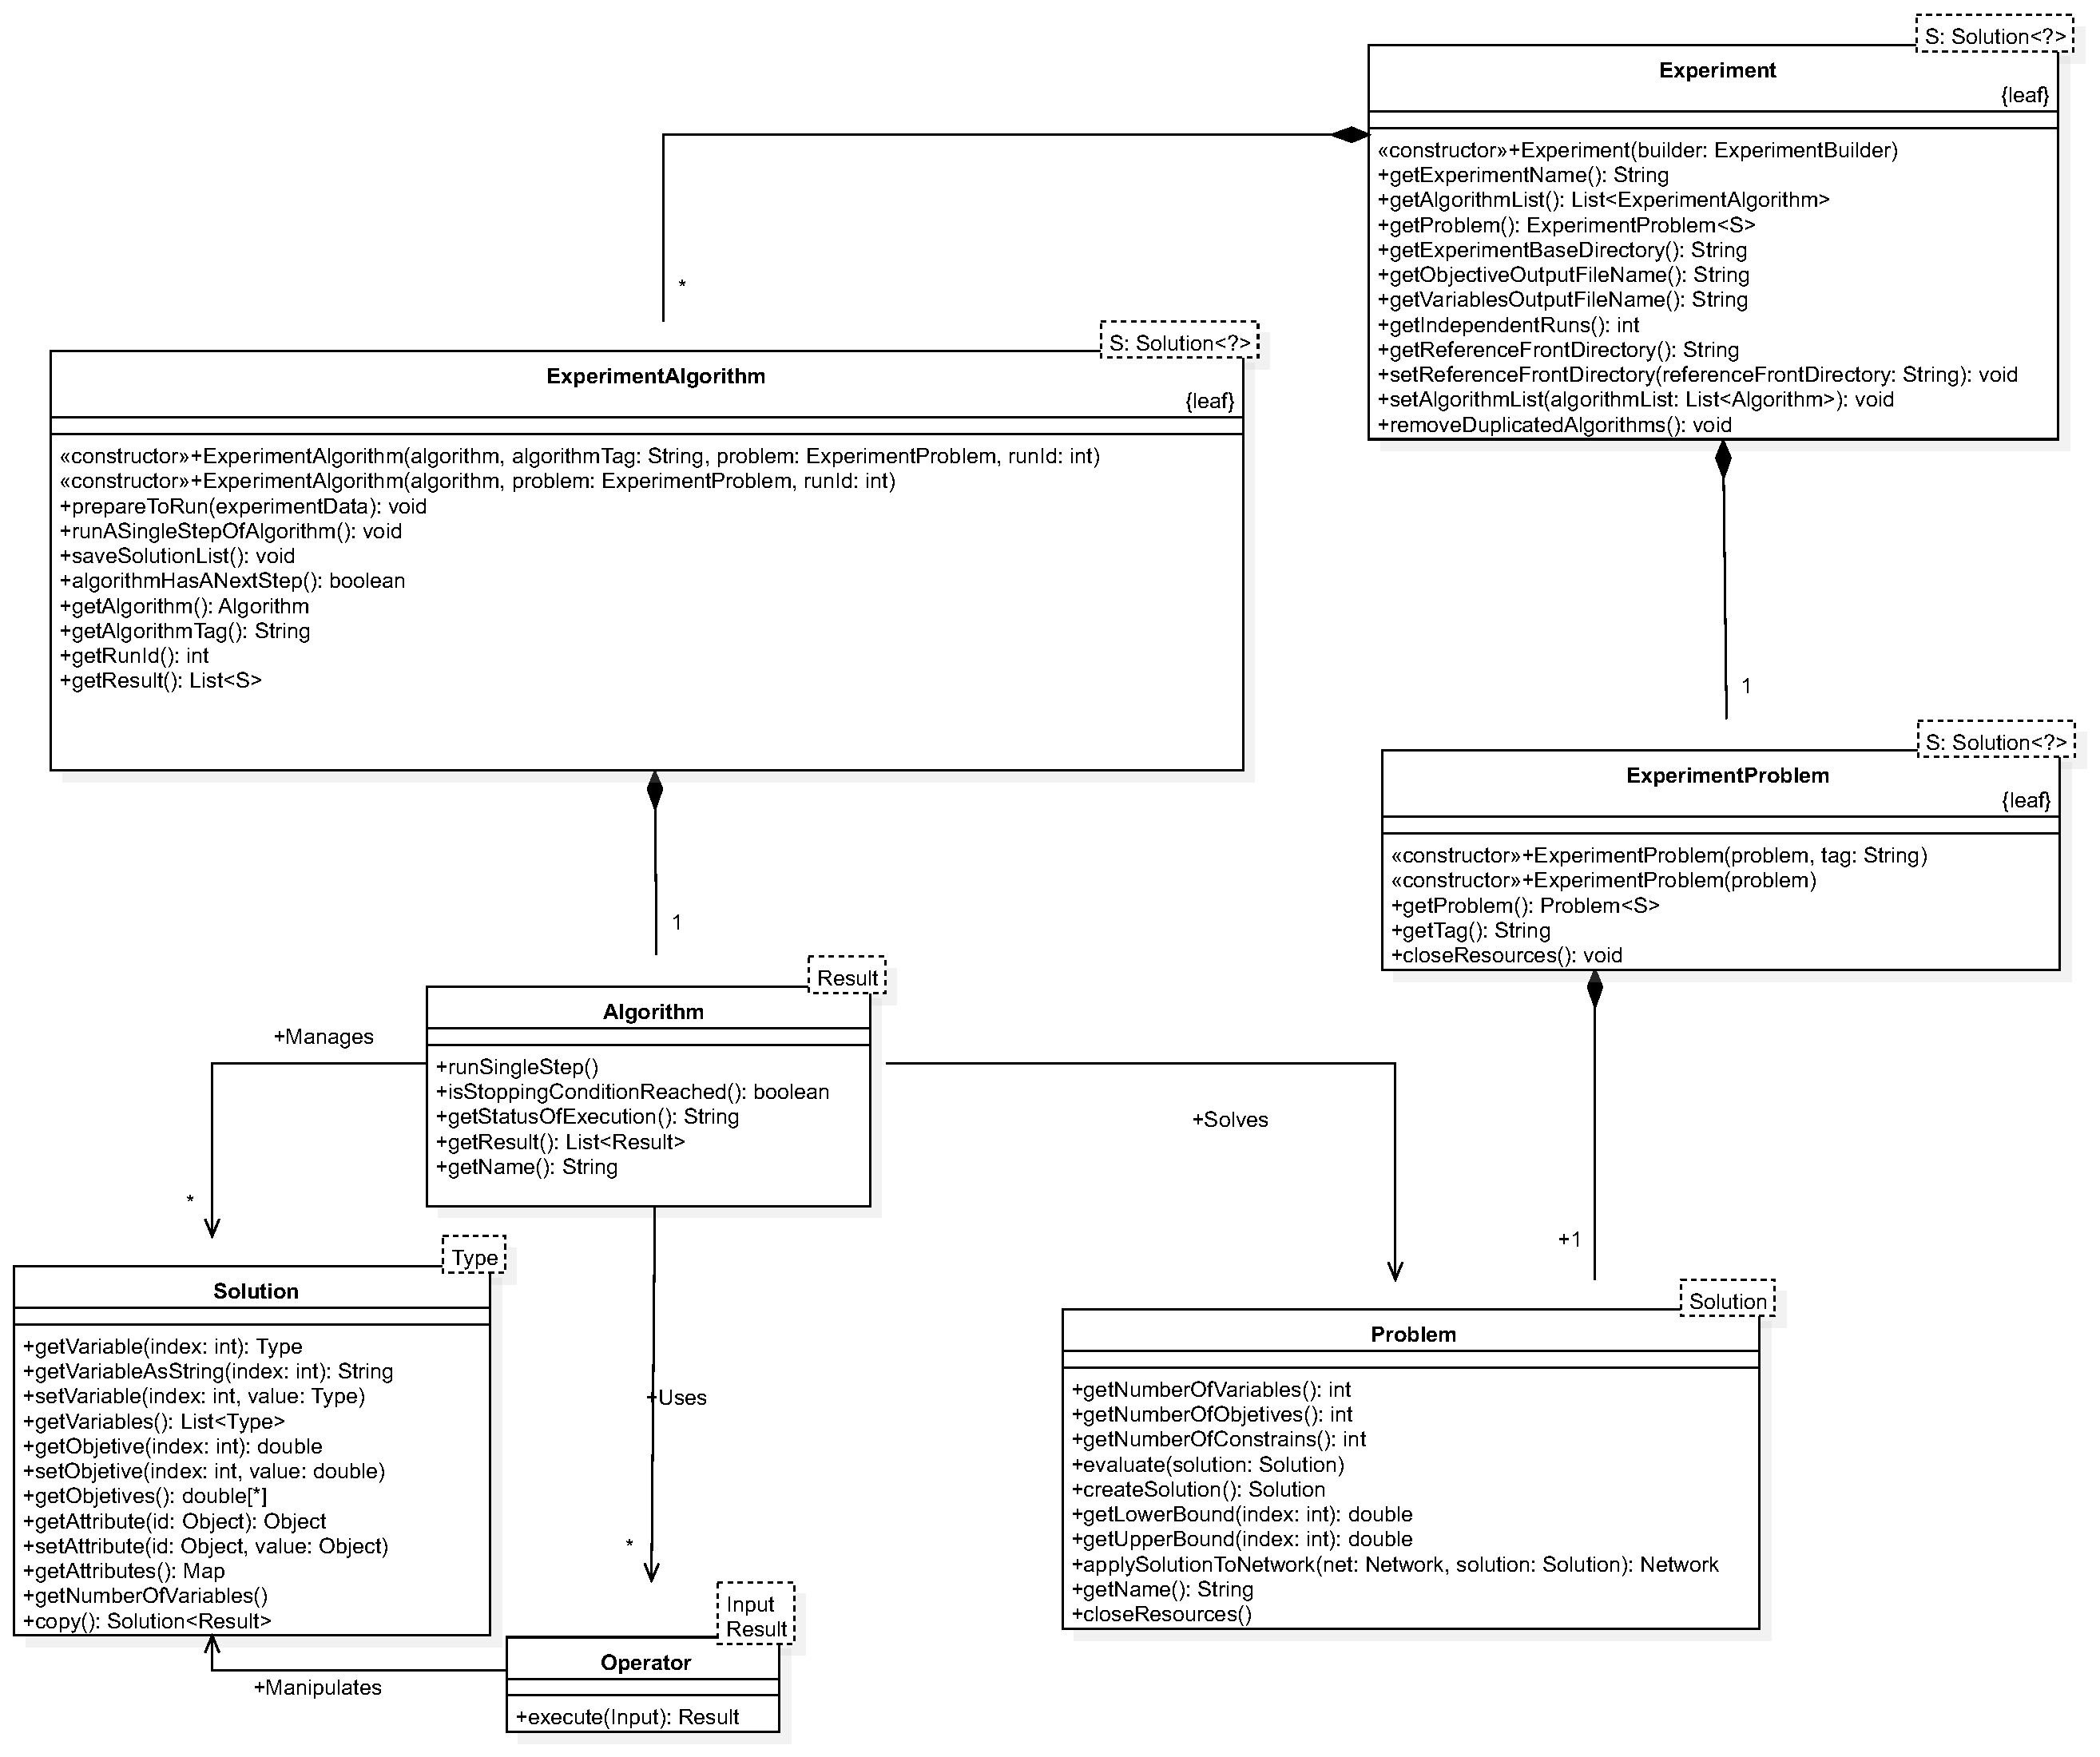
\includegraphics[width=\textwidth]{Capitulo3/assets/module_metaheuristic.eps}
    \caption{Diagrama de clases del componente \textit{metaheuristic}.}
    \label{fig:module_metaheuristic}
\end{figure}    